\documentclass{beamer}
\usepackage{graphicx}
\usepackage{tikz}
\usetikzlibrary{shapes,arrows}
\usepackage{tikz}
%\usecolortheme{seahorse}
  \setbeamertemplate{footline}[page number]
\usepackage{multirow}
\setbeamertemplate{navigation symbols}{}
\setbeamertemplate{frametitle}[default][center]
\setbeamerfont{frametitle}{shape=\scshape}
\usepackage{color}

\usepackage{csquotes}

\usepackage{xcolor}

\usepackage[flushleft]{threeparttable}

{\title{\textsc{Econ 352 - Consumer and Firm Behavior: The Work-Leisure Decision and Profit Maximization} \\ \tiny (See Williamson Ch. 4)}
\author{Trevor S. Gallen}
\date{}
\begin{document}
\renewcommand*{\inserttotalframenumber}{\pageref{lastframe}}


\setbeamertemplate{caption}{\raggedright\insertcaption\par}

\begin{frame}
\titlepage
\end{frame}

\begin{frame}
\frametitle[alignment=center]{The Beginning}
\begin{itemize}
\item Finally, we're going to start building up a model
\bigskip
\item This model will look a lot like what you learn in micro!  
\bigskip
\item Start in a ``static" (unmoving, one-period) model, then eventually go to ``dynamic" (multi-period)
\bigskip
\item We'll build up a basic consumer that chooses how much to consume (work), and how much to leisure (not work)
\bigskip
\item Then we'll build up a firm that uses labor and capital to produce a consumption good
\bigskip
\item In Chapter 5, we'll then put those two together to create a ``representative agent" macroeconomy
\end{itemize}
\end{frame}

\begin{frame}
\frametitle[alignment=center]{Representative Consumer}
\begin{itemize}
\item Start with a representative consumer
\bigskip
\item Consumer likes consumption $C$ and likes leisure $\ell$
\bigskip
\item The two inputs map into happiness (utility) $U(C,\ell)$
\bigskip
\item  Call a particular $(C_1,\ell_1)$ combination a ``consumption bundle"
\bigskip
\item Bundle $(C_1,\ell_1)$ is ``strictly preferred" to bundle $(C_2,\ell_2)$ if:
$$U(C_1,\ell_1)>U(C_2,\ell_2)$$
\item A consumer is ``indifferent" between bundles  $(C_1,\ell_1)$ and $(C_2,\ell_2)$ if:
$$U(C_1,\ell_1)=U(C_2,\ell_2)$$
\item Now we'll think about the properties of consumer preferences
\end{itemize}
\end{frame}

\begin{frame}
\frametitle[alignment=center]{Representative Consumer-Principles}
\begin{itemize}
\item We have a few beliefs about the consumer
\begin{enumerate}
\item More is always preferred to less: $U(C_1,\ell_1)<U(C_1+\epsilon,\ell_1)$ and $U(C_1,\ell_1)<U(C_1,\ell_1+\epsilon)$, $\epsilon>0$ (normal goods)
\bigskip
\item Consumer likes diversity: take some optimal $(C^*,\ell^*)$ bundle.  Then $U(\frac{1}{2}C^*,2\ell^*)>U(\frac{1}{4}C^*,4\ell^*)$  (imperfect substitution)
\bigskip
\item Consumption and leisure are normal goods: as income increases, people want more of both consumption and leisure
\begin{itemize}
\item Goods are ``luxury" if you consume relatively more of them as income increases
\item Goods are ``normal" if you consume more of them as income increases (even if share of spending falls)
\item Goods are ``inferior" if you consume less of them as income increases
\end{itemize}
\item Let's think about the all-important ``indifference curve"
\end{enumerate}
\end{itemize}
\end{frame}




\begin{frame}
\frametitle[alignment=center]{Indifference Curves}
\begin{itemize}
\item Indifference curves are the curves along which a person is indifferent to one bundle or another.  So, for some utility level $\bar{U}$, the indifference curve is defined over C and L by $\bar{U}=U(C,\ell)$.
\bigskip
\item For instance, let's say you have 1.5 units of happiness from working 1 hour and consuming 3 candy bars.  $U(3,1)=1.5=\bar{U}$.  The indifference curve tells us the set of bundles that would make you just as happy.  For instance, if you had to deviate to leisuring only 0.5 hours, you might require not six but \emph{seven} candy bars $U(7,0.5)=1.5$.  
\bigskip
\item Let's think about two indifference curves defined by $U(C,\ell)=I_1$ and  $U(C,\ell)=I_2$
\end{itemize}
\end{frame}

\begin{frame}
\frametitle[alignment=center]{Indifference Curves}
\begin{figure}
\centering
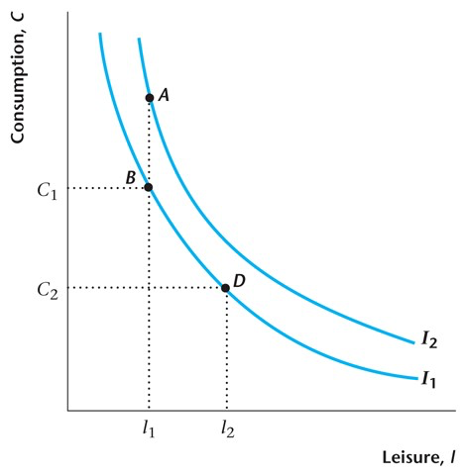
\includegraphics[scale=0.5]{Figures/W_Fig_4pt1.png}
\end{figure}
$U(C_B,\ell_B)=U(C_D,\ell_D)<U(C_A,\ell_A)$\\
Notice the bow/curve!
\end{frame}

\begin{frame}
\frametitle[alignment=center]{Properties of Indifference Curves}
\begin{figure}
\centering
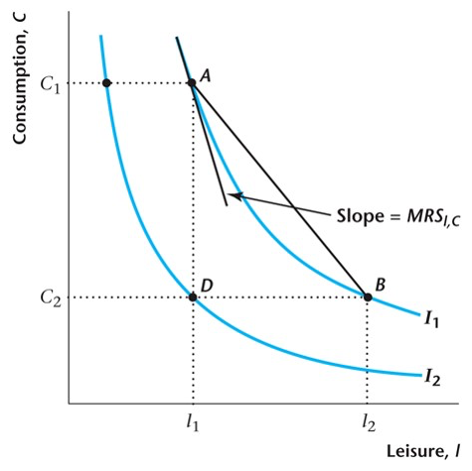
\includegraphics[scale=0.5]{Figures/W_Fig_4pt2.png}
\end{figure}
MRS=slope=willingness to trade off (price at which indifferent!)
\end{frame}

\begin{frame}
\frametitle[alignment=center]{Budget Constraint}
\begin{itemize}
\item Now we know how the consumer feels about various bundles
\bigskip
\item But how do they decide? Constrained optimization (otherwise choose infinite amounts!)
\bigskip
\item Need a \textbf{budget constraint}
\bigskip
\item Assume consumer is in a competitive market (I assume my wage is given/I can't change it)
\end{itemize}
\end{frame}

\begin{frame}
\frametitle[alignment=center]{Budget Constraint-II}
\begin{itemize}
\item Time constraint, letting $\ell$ be leisure, $N^s$ be work time, and $h$ be total free hours:
$$\ell+N^s=h$$
\item Great, $h$ is some fixed amount, $\ell$ is leisure, but where does $N^s$ play into all this?
\bigskip
\item Workers get paid some real wage $w$ for their hourly work, which they can use to buy $C$ (trade off between $\ell$ and $C$ now, via $N^s$!
\end{itemize}
\end{frame}

\begin{frame}
\frametitle[alignment=center]{Budget Constraint-II}
\begin{itemize}
\item Letting $N^S$ be work time, $w$ be the real wage, $\pi$ be ``dividend income" and T be ``lump-sum" tax:
$$C=wN^s+\pi-T$$
\item Then, plugging in the time budget constraint:
$$C=w(h-\ell)+\pi-T$$
\item Or:
$$C+w\ell=\underbrace{wh+\pi-T}_{\text{Disposable ``income"}}$$
\item Let's graph out the budget constraint in terms of $C$ as a function of $\ell$:
$$C=\underbrace{wh+\pi-T}_{\text{Intercept}}\underbrace{-w}_{\text{Slope}}\ell$$
\end{itemize}
\end{frame}

\begin{frame}
\frametitle[alignment=center]{BC when $T>\pi$}
\begin{figure}
\centering
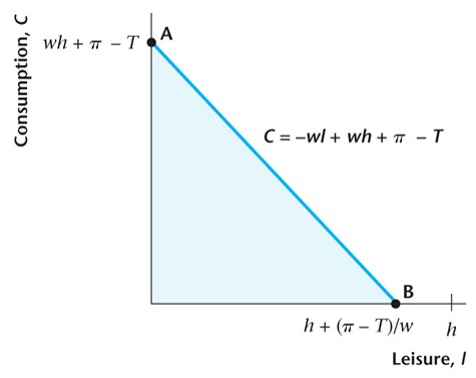
\includegraphics[scale=0.5]{Figures/W_Fig_4pt3.png}
\end{figure}
\end{frame}

\begin{frame}
\frametitle[alignment=center]{BC when $T<\pi$}
\begin{figure}
\centering
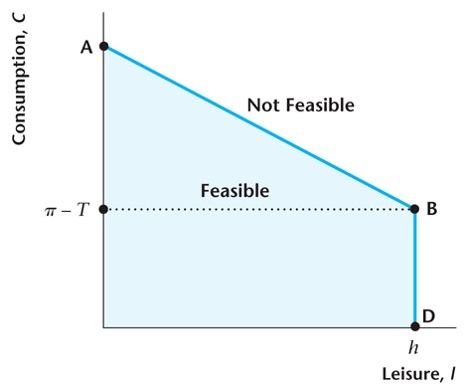
\includegraphics[scale=0.5]{Figures/W_Fig_4pt4.png}
\end{figure}
\end{frame}

\begin{frame}
\frametitle[alignment=center]{How does consumer optimize?}
\begin{itemize}
\item Wants the highest possible indifference curve that fits along the budget constraint
\bigskip
\item Intuitively, the indifference curve will just barely ``kiss" the budget constraint
\bigskip
\item If it didn't you could improve utility by moving up and to the right (increase both leisure and consumption)
\end{itemize}
\end{frame}

\begin{frame}
\frametitle[alignment=center]{Consumer optimization}
\begin{figure}
\centering
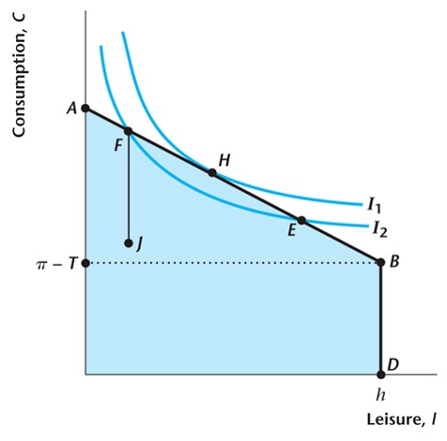
\includegraphics[scale=0.5]{Figures/W_Fig_4pt5.png}
\end{figure}
F is better than J, E is the same as F, but H is the best
\end{frame}

\begin{frame}
\frametitle[alignment=center]{In math}
\begin{itemize}
\item Constrained optimization problem (Lagrangian):
$$U(C,\ell)+\lambda(wh+\pi-T-w\ell)$$
\item Unconstrained optimization problem:
$$U(wh+\pi-T-w\ell,\ell)$$
\item Optimum happens when $\frac{\partial U}{\partial \ell}=0$
$$-wU(C^*,\ell^*)+U_2(C^*,\ell^*)=0$$
\item Or:
$$w=-\frac{U_2(C^*,\ell^*)}{U_1(C^*,\ell^*)}$$
\item But note that along $U(C,\ell)=\bar{U}$:
$$\frac{d C}{d \ell}|_{U(C,\ell)=\bar{U}}=-\frac{\frac{\partial U}{\partial \ell} }{\frac{\partial U}{\partial C}}=w$$
\item The best indifference curve is tangent to our budget constraint (has slope -w wrt $N^s$)
\end{itemize}
\end{frame}

\begin{frame}
\frametitle[alignment=center]{At the optimum}
\begin{itemize}
\item At the (interior!) optimum, we know that $MRS_{\ell,C}=w$
\bigskip
\item Marginal rate of substitution of leisure for consumption is the wage
\bigskip
\item If you were had to work one more hour, you would have to get $w$ more consumption to be indifferent (at optimum, indifferent between more labor and more consumption, or less labor and less consumption)
\bigskip
\item Now we'll have some predictions, which we'll mostly think of graphically
\end{itemize}
\end{frame}

\begin{frame}
\frametitle[alignment=center]{Consumer optimization}
\begin{figure}
\centering
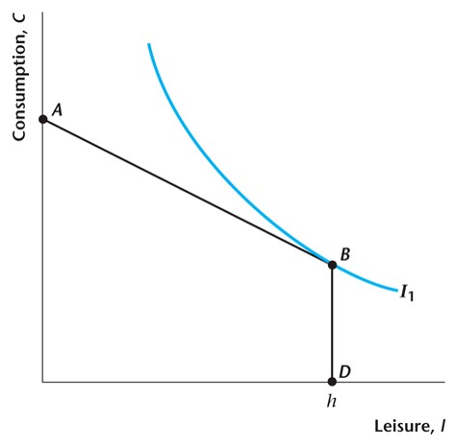
\includegraphics[scale=0.5]{Figures/W_Fig_4pt6.png}
\end{figure}
We could be at a ``corner solution"
\end{frame}


\begin{frame}
\frametitle[alignment=center]{Changes in Real Dividends or Taxes}
\begin{itemize}
\item Now let's think about a change in $\pi-T$, the ``property income"
\bigskip
\item Such a change is a ``pure income effect" because it affects income but not the budget-constraint tradeoff between labor and leisure
\bigskip
\item If leisure and consumption are both normal goods, then both should increase when $\pi-T$ increases
\end{itemize}
\end{frame}

\begin{frame}
\frametitle[alignment=center]{Non-labor income increase}
\begin{figure}
\centering
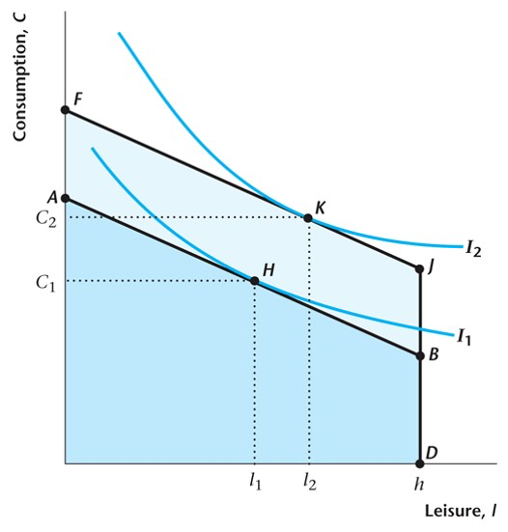
\includegraphics[scale=0.5]{Figures/W_Fig_4pt7.png}
\end{figure}
``Pure income effect:" consume more of everything ($c\uparrow$, $\ell\uparrow$, $N\downarrow$)
\end{frame}


\begin{frame}
\frametitle[alignment=center]{Changes in the Real Wage}
\begin{itemize}
\item Changes in the real wage $w$ are far more complicated
\bigskip
\item If your wage increased, would you work more or less?
\begin{itemize}
\item On one hand, leisure is a normal good, I'm richer, work less  (``income effect")
\item On other hand, consumption is now ``cheaper" in terms of labor, consume more of that! (``substitution effect")
\end{itemize}
\item We call the substitution effect how we would change leisure if we were constrained to be on the same utility curve (no increase in ``income" (happiness))
\item We call the income effect the residual left over: the effect of moving to our higher indifference curve after the substitution effect
\item Let's see it graphically
\end{itemize}
\end{frame}

\begin{frame}
\frametitle[alignment=center]{Wage Increase}
\begin{figure}
\centering
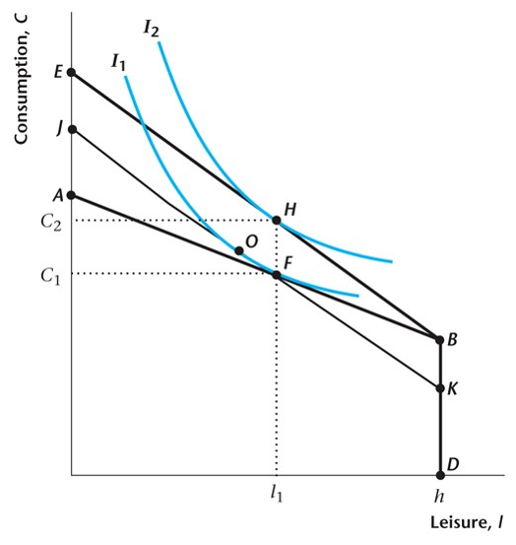
\includegraphics[scale=0.5]{Figures/W_Fig_4pt8.png}
\end{figure}
When wages increase from B-A to B-E, define $F\rightarrow O$ as ``substitution effect" and $O\rightarrow H$ as ``income effect."  K-J is the change in wage but no change in ``income" (utility curve), which gives substitution effect.
\end{frame}

\begin{frame}
\frametitle[alignment=center]{Labor supply curve}
\begin{itemize}
\item While what we do builds from indifference curves, we sometimes use the result of them, the ``labor supply curve"
$$N^s(w)=h-\ell(w)$$
\item Ordinarily, we think that the labor supply curve slopes upward (substitution effect dominates)
\bigskip
\item While we'll talk about why, it's primarily because we're talking about short run changes in the wage that mostly mute the substitution effect (dynamics we haven't yet seen)
\bigskip
\item But we'll see!  In long run, it may be that income effect dominates substitution!
\bigskip
\item But mostly, they're relatively close to balancing (``balanced growth preferences")
\end{itemize}
\end{frame}


\begin{frame}
\frametitle[alignment=center]{Labor supply curve}
\begin{figure}
\centering
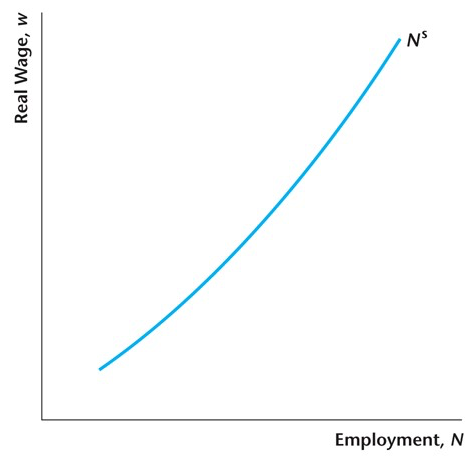
\includegraphics[scale=0.5]{Figures/W_Fig_4pt9.png}
\end{figure}
\end{frame}


\begin{frame}
\frametitle[alignment=center]{Effect of property income increase on labor supply}
\begin{figure}
\centering
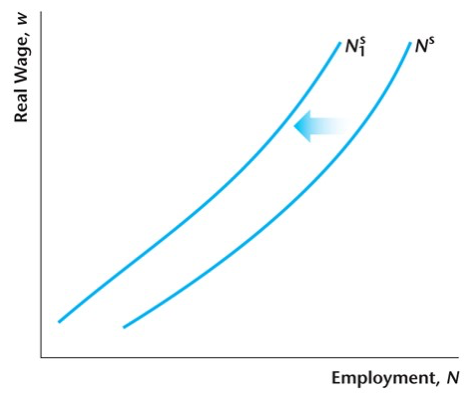
\includegraphics[scale=0.5]{Figures/W_Fig_4pt10.png}
\end{figure}
\end{frame}

\begin{frame}
\frametitle[alignment=center]{Closed-Form Solution}
\begin{itemize}
\item Let's take the following example (Williamson does perfect complements in book):
$$U(C,\ell)=log(C)+\psi log(\ell)$$
\item Such that: $C=wh+\pi-T-w\ell$
\item Can write the Lagrangian as:
$$\mathcal{L}=\max{C,\ell}\left\{log(C)+\psi \log(\ell)+\lambda\left(wh+\pi-T-C-w\ell\right)\right\}$$
FOC's:
$$\frac{1}{C^*}=\lambda^*$$
$$\frac{\psi}{w\ell^*}=\lambda^*$$
$$wh+\pi-T=C^*+w\ell^*$$
Solving these three equations for three unknowns ($C^*,\ell^*,\lambda^*$):
$$C^*=\frac{\pi-T+hw}{1+\psi}\ \ \ \ \ell^*=\frac{\psi}{1+\psi}\frac{hw+\pi-T}{w}$$
\item Can see that when $\pi-T\uparrow$, $C^*\uparrow$, and $\ell^*\uparrow$
\end{itemize}
\end{frame}

\begin{frame}
\frametitle[alignment=center]{Taking Stock}
\begin{itemize}
\item Okay, great, we have the ``representative agent"/``representative consumer"
\bigskip
\item But where do wages and consumption goods come from?  
\bigskip
\item The ``representative firm" 
\bigskip
\item Representative firm will have a \textbf{production function} that takes in capital $K$ and labor demanded $N^d$:
$$Y=zF(K,N^d)$$
\item We call $z$ the ``total factor productivity
\item Crucial to understanding firm behavior is the \textbf{marginal product}.
\item The marginal product of a factor of production is the additional output that can be produced with one additional unit of that factor input, holding constant the quantities of other factor inputs (e.g. MPL would be $\frac{\partial Y(K,N^d)}{\partial N^d}$, how much more $Y$ you get if you add a unit of $N^d$ holding $K$ constant)
\end{itemize}
\end{frame}

\begin{frame}
\frametitle[alignment=center]{Properties of the production function}
\begin{itemize}
\item As we did with the consumer, we start with five sensible properties
\begin{enumerate}
\item Production function exhibits constant returns to scale (double inputs, double outputs):
$$zF(xK,xN^d)=xzF(K,N^d)$$
\item Output increases when either capital input or the labor input increases:
$$\frac{\partial F(K,N^d)}{\partial K}>0\ \ \ \text{and} \ \ \ \frac{\partial F(K,N^d)}{\partial N^d}>0$$
\item The marginal product of labor decreases as the amount of labor increases:
$$\frac{\partial^2 F(K,N^d)}{\partial (N^d)^2}<0$$
\end{enumerate}
\end{itemize}
\end{frame}

\begin{frame}
\frametitle[alignment=center]{Properties of the production function-II}
\begin{enumerate}\addtocounter{enumi}{3}
\item The marginal product of capital decreases as the amount of capital increases:
$$\frac{\partial^2 F(K,N^d)}{\partial (N^d)^2}<0$$
\item The marginal product of capital increases as the amount of labor increases, and the marginal product of labor increases as the amount of capital increases:
$$\frac{\partial^2 F(K,N^d)}{\partial (N^d)\partial K}=\frac{\partial^2 F(K,N^d)}{\partial K \partial (N^d)}>0$$
\end{enumerate}
\end{frame}



\begin{frame}
\frametitle[alignment=center]{Production Function, fixing Capital and Varying Labor}
\begin{figure}
\centering
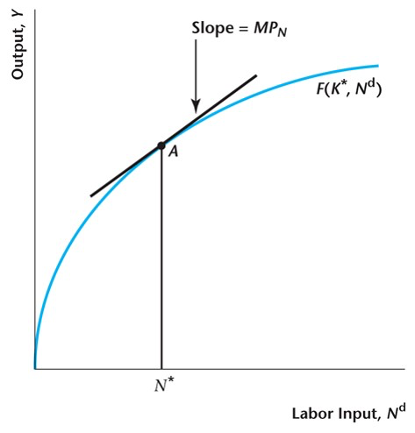
\includegraphics[scale=0.5]{Figures/W_Fig_4pt12.png}
\end{figure}
Note x-axis is capital
\end{frame}

\begin{frame}
\frametitle[alignment=center]{Production Function, fixing Labor and Varying Capital}
\begin{figure}
\centering
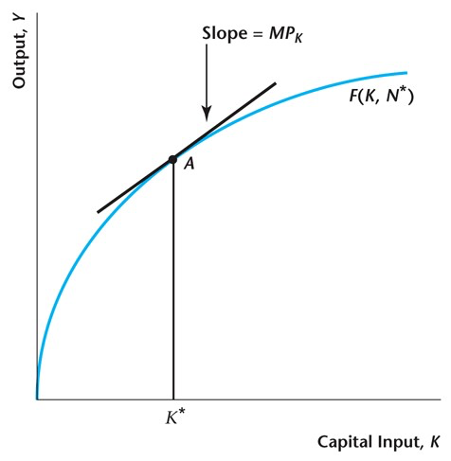
\includegraphics[scale=0.5]{Figures/W_Fig_4pt13.png}
\end{figure}
Note x-axis is labor
\end{frame}

\begin{frame}
\frametitle[alignment=center]{Marginal Product of Labor as Function of Labor}
\begin{figure}
\centering
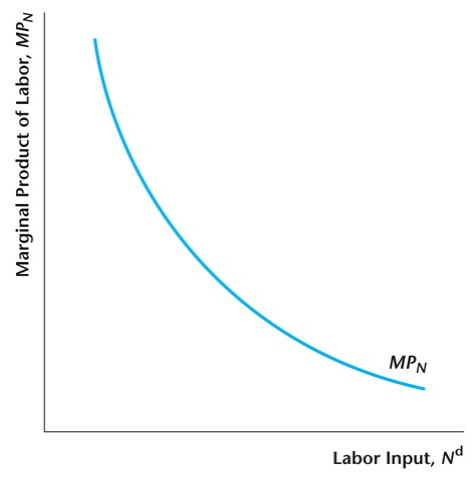
\includegraphics[scale=0.5]{Figures/W_Fig_4pt14.png}
\end{figure}
Labor is less productive as you get more of it (holding capital constant)
\end{frame}

\begin{frame}
\frametitle[alignment=center]{Marginal Product of Labor as Function of Labor, increasing Capital}
\begin{figure}
\centering
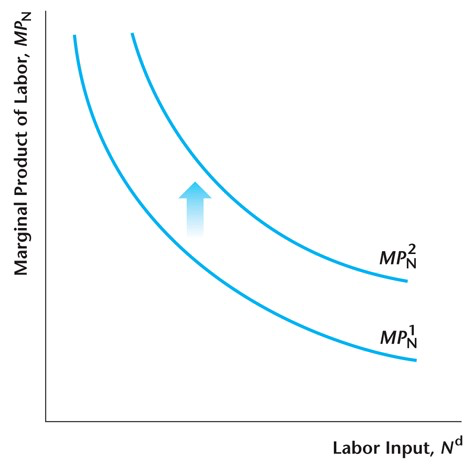
\includegraphics[scale=0.5]{Figures/W_Fig_4pt15.png}
\end{figure}
Marginal product of labor shifts up when capital increases
\end{frame}

\begin{frame}
\frametitle[alignment=center]{Total factor productivity increase on output as a function of labor}
\begin{figure}
\centering
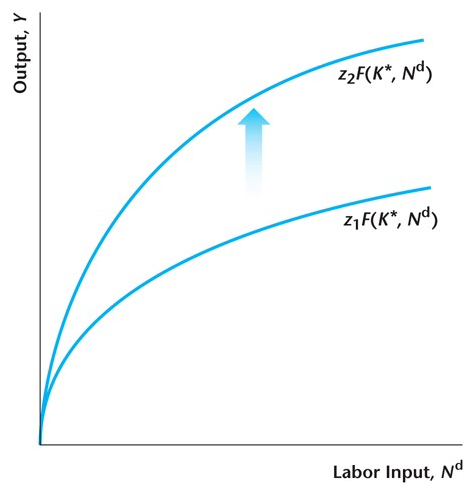
\includegraphics[scale=0.5]{Figures/W_Fig_4pt16.png}
\end{figure}
\end{frame}

\begin{frame}
\frametitle[alignment=center]{Total factor productivity increase on MPL as a function of labor}
\begin{figure}
\centering
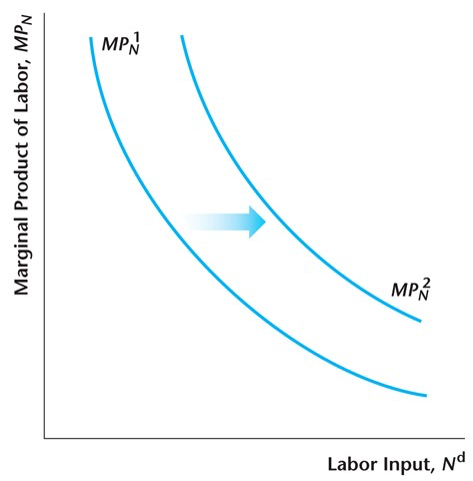
\includegraphics[scale=0.5]{Figures/W_Fig_4pt17.png}
\end{figure}
\end{frame}

\begin{frame}
\frametitle[alignment=center]{Profit Maximization}
\begin{itemize}
\item We assume that firms choose  $K$ and $N^d$ to maximize profit $\pi$:
$$\pi=zF(K,N^d)-wN^d-rK$$
\item When choosing how much labor to use, take FOC with respect to labor (assume wage is given!):
$$\frac{\partial \pi(K,N^d)}{\partial N^d}=0$$
\item Or:
$$z\frac{\partial F(K,N^d)}{\partial N^d}-w=0$$
\item Or, the marginal product of labor is equal to the wage:
$$MP_N=w$$
\end{itemize}
\end{frame}

\begin{frame}
\frametitle[alignment=center]{Revenue, variable costs, and profit maximization}
\begin{figure}
\centering
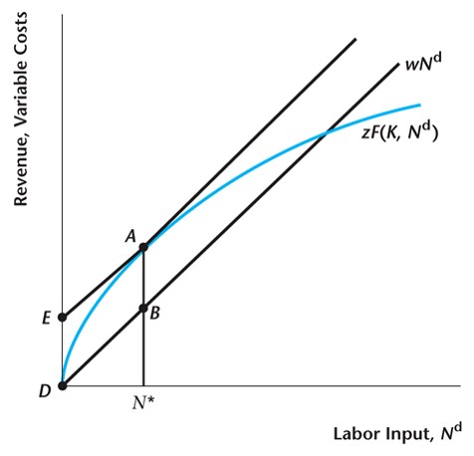
\includegraphics[scale=0.5]{Figures/W_Fig_4pt19.png}
\end{figure}
\end{frame}


\begin{frame}
\frametitle[alignment=center]{Marginal product of labor curve is labor demand curve}
\begin{figure}
\centering
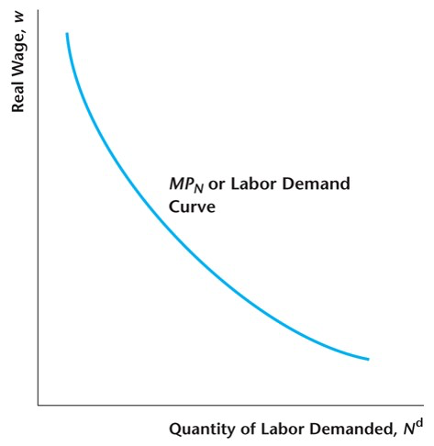
\includegraphics[scale=0.5]{Figures/W_Fig_4pt20.png}
\end{figure}
\end{frame}


\begin{frame}
\frametitle[alignment=center]{Measuring Z, the Solow Residual}
\begin{itemize}
\item $z$ is a measure of all the things we don't know and/or didn't model
\bigskip
\item We can measure it for a specific production function if we know $K$, $N^d$, $Y$, and have the production function.  For instance, if:
$$Y=zK^0.3L^{0.7}$$
\item Then can measure $z$ as:
$$z^{measured}=\frac{Y^{data}}{(K^{data})^0.3(L^{data})^{0.7}}=\frac{z^{true}K^{data})^0.3(L^{data})^{0.7}}{(K^{data})^0.3(L^{data})^{0.7}}=z^{true}$$
\item Note that if true reality is actually: $Y=z^{true}K^{0.3}L^{0.7}O^{0.1}$ then:
$$z^{measured}=\frac{z^{true}K^{0.3}L^{0.7}O^{0.1}}{(K^{data})^{0.3}(L^{data})^{0.7}}=z^{true}O^{0.1}$$
\item So the residual will move with not only the true residual but also O (oil).  
\end{itemize}
\end{frame}

\begin{frame}
\frametitle[alignment=center]{Solow Residual}
\begin{figure}
\centering
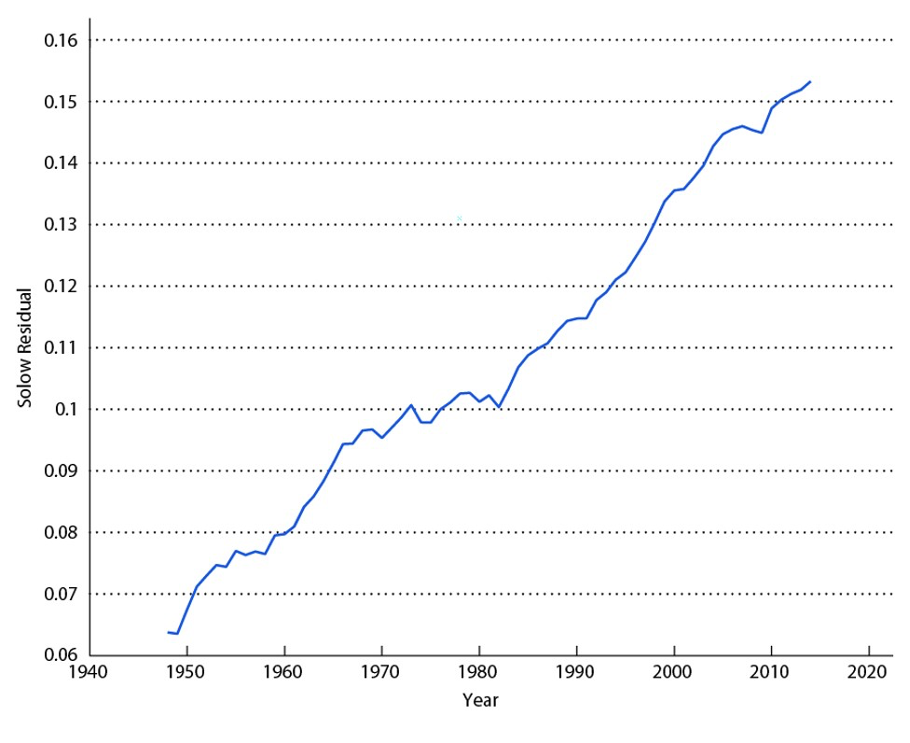
\includegraphics[scale=0.5]{Figures/W_Fig_4pt18.png}
\end{figure}
\end{frame}


\begin{frame}
\frametitle[alignment=center]{Fernald ``Solow" Residual}
\begin{figure}
\centering
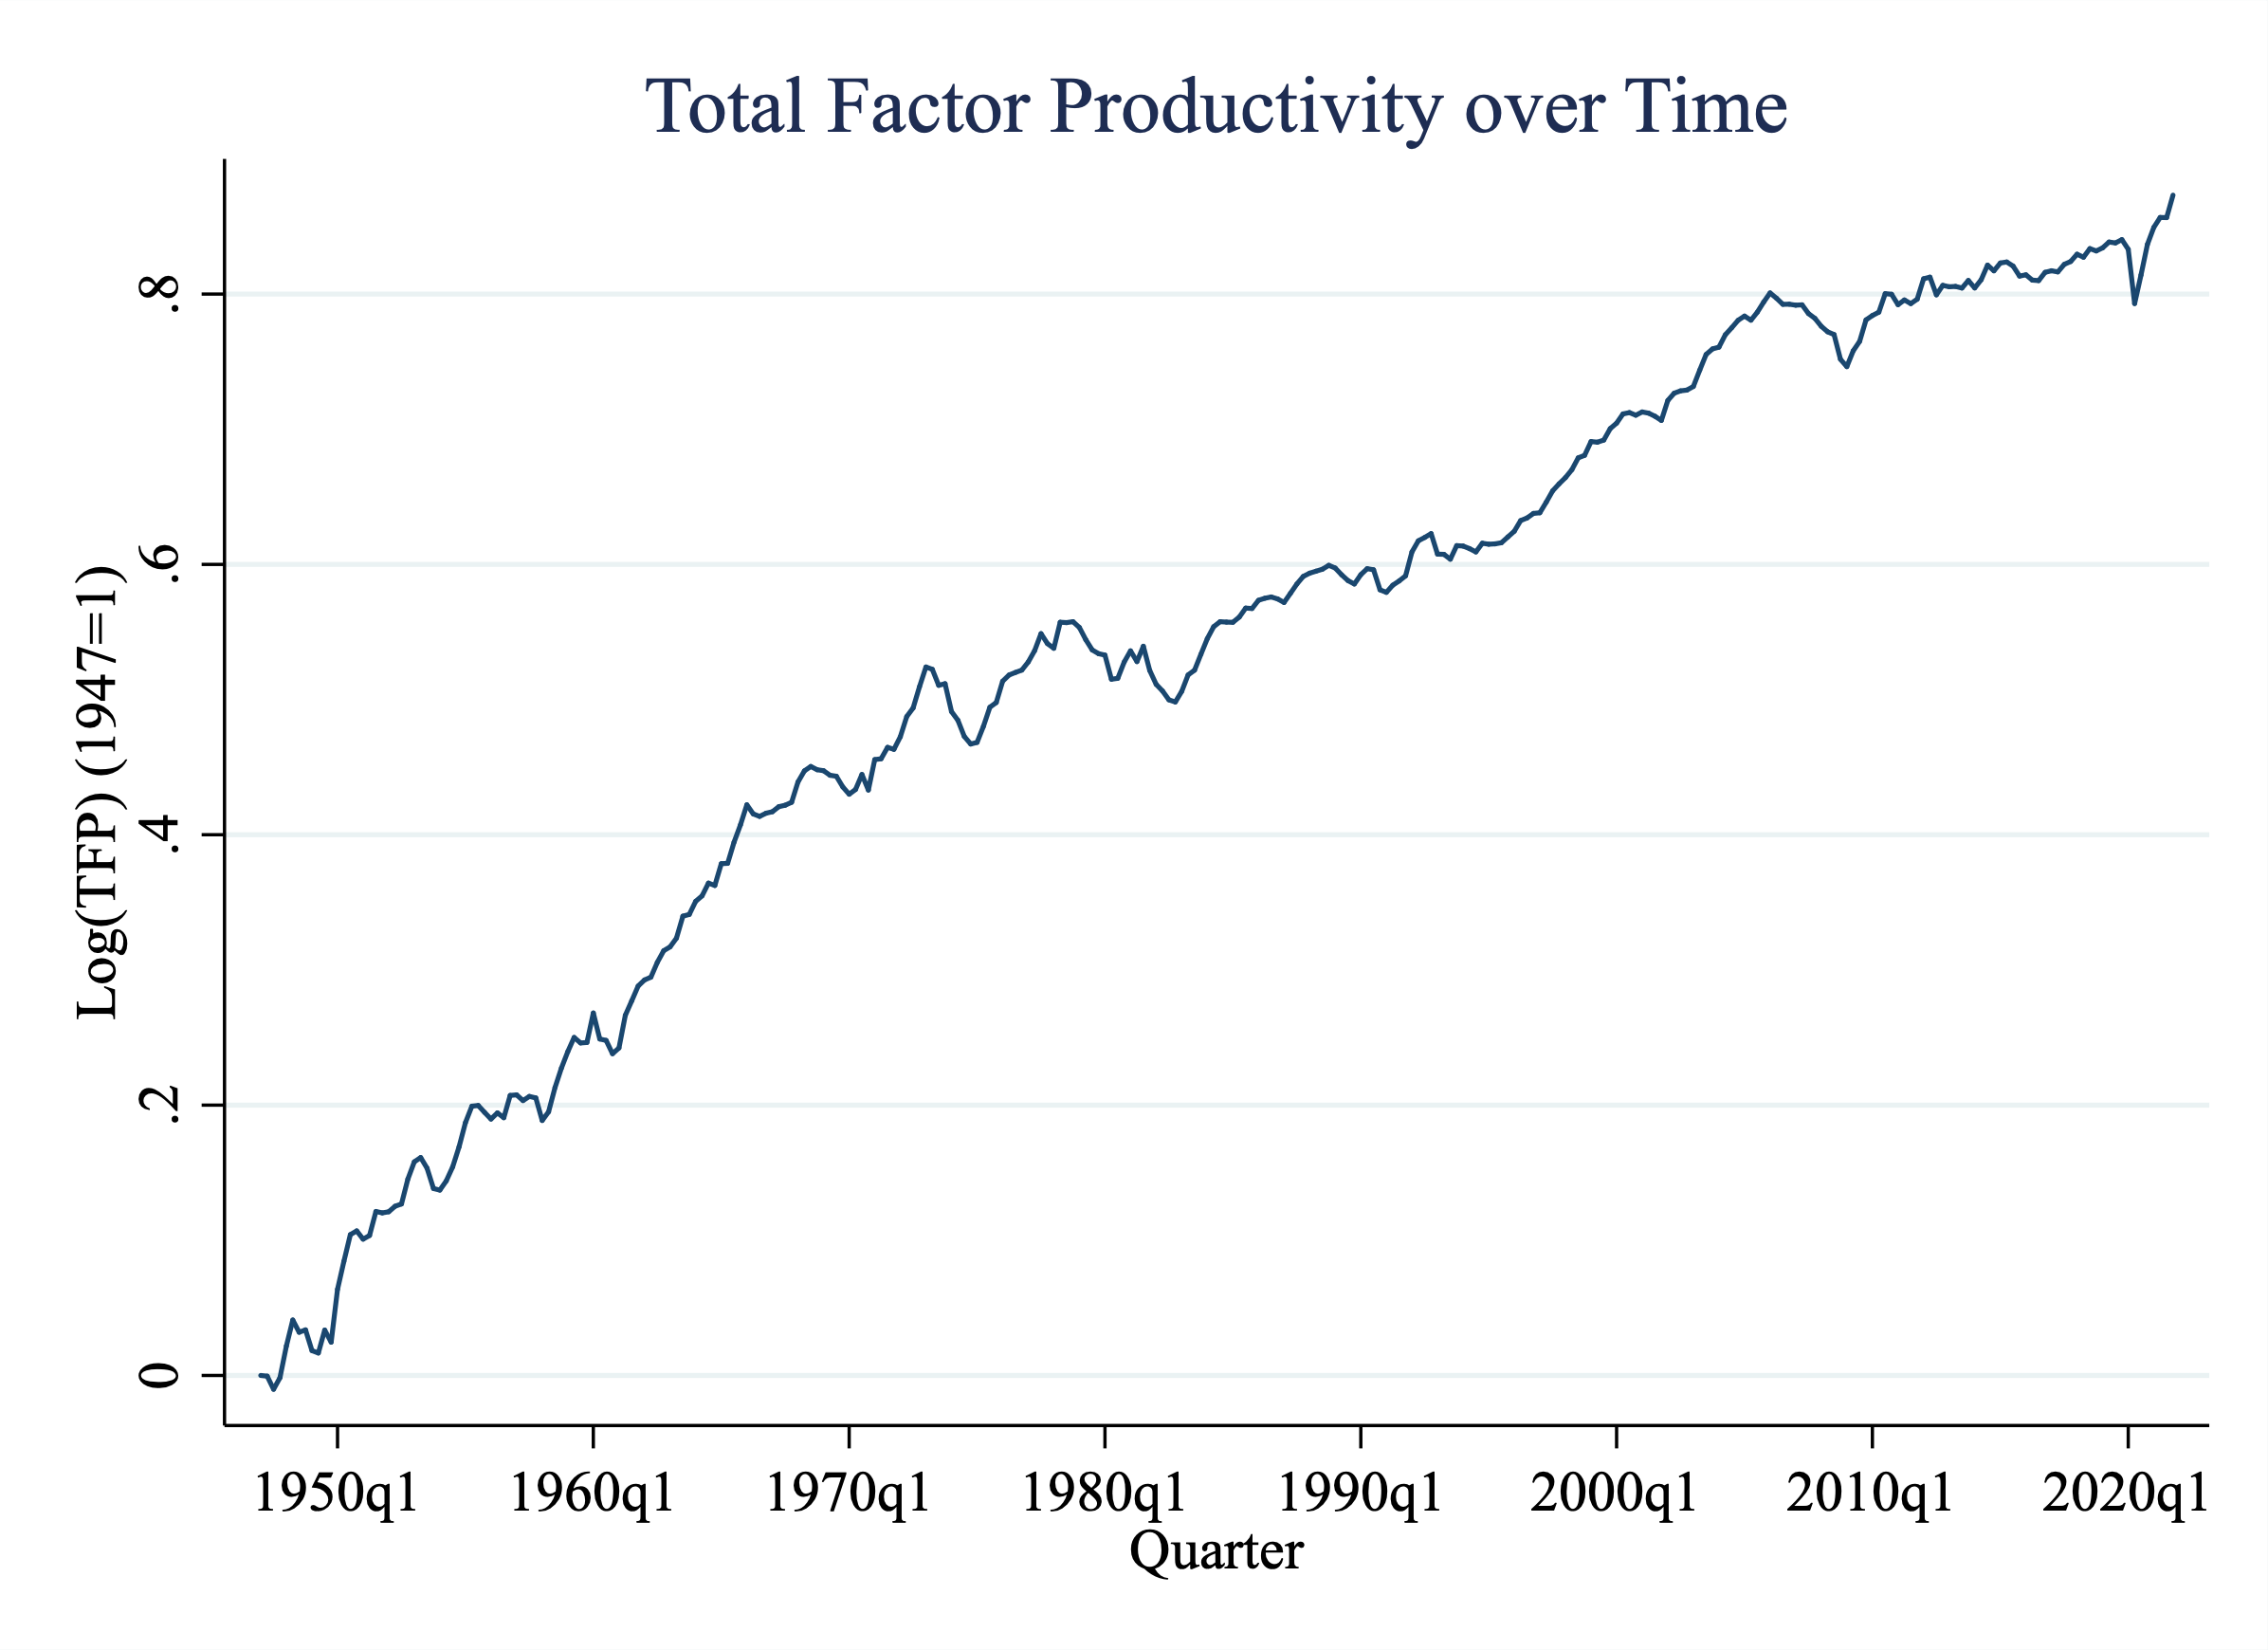
\includegraphics[scale=0.2]{Figures/Fernald_TFP.png}
\end{figure}
Adjusts for inputs such as capital utilization, labor composition (richer model, like modeling oil above)
\end{frame}



\begin{frame}
\frametitle[alignment=center]{Next Steps}
\begin{itemize}
\item Now, we have a consumer and a producer, we want to ``close" the model, which we'll do next chapter
\bigskip
\item This ``closing" will be a big distinction from micro/labor
\end{itemize}
\end{frame}




\end{document}